\textbf{(Challenge Question)} (\textit{Exercise 4.4 S\&B)} The policy iteration algorithm on page 80 has a subtle bug in that it may never terminate if the policy continually switches between two or more policies that are equally good. This is ok for pedagogy, but not for actual use. Modify the pseudocode so that convergence is guaranteed. Note that there is more than one approach to solve this problem. 

\begin{figure}[h!]
\centering
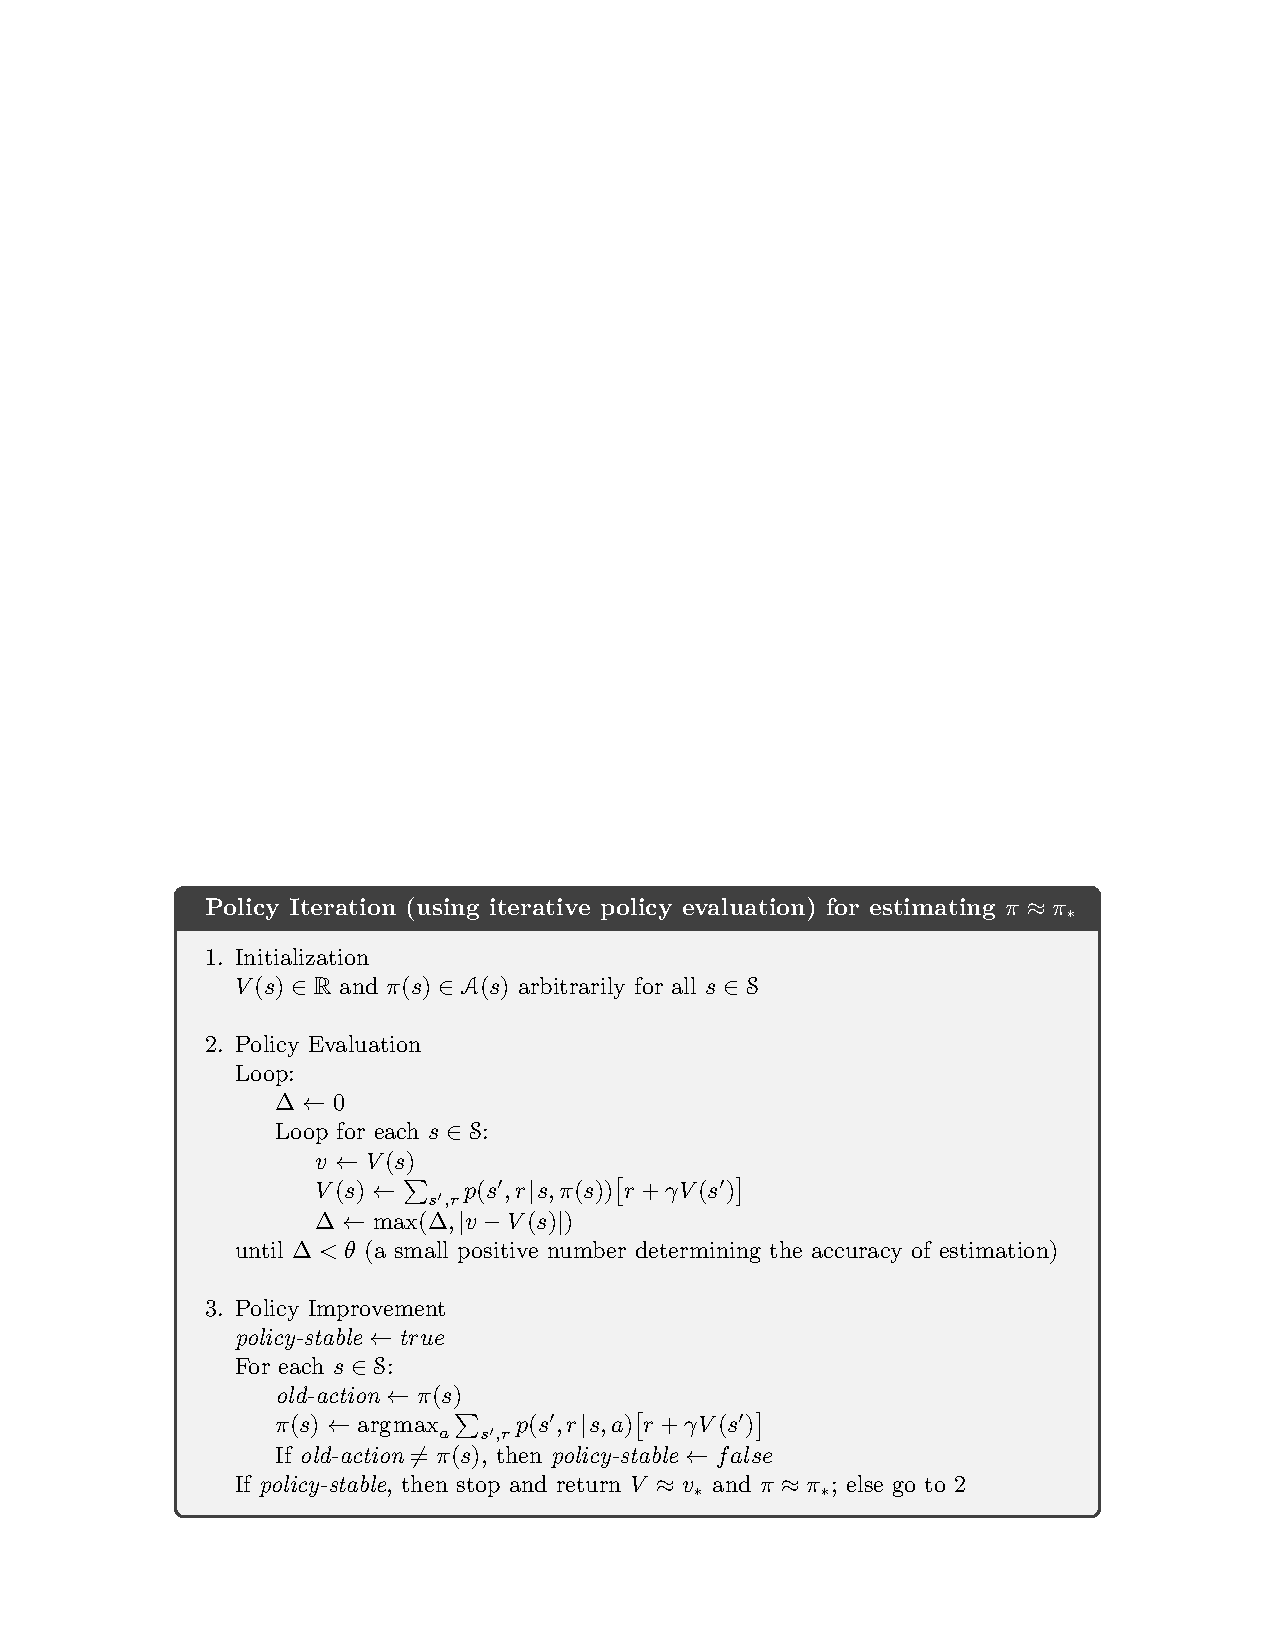
\includegraphics[scale=0.9]{figures/pseudocode_pi.pdf}
\end{figure}